\chapter{EPI-to-EPI inter-subject nonlinear registration}\label{chap:epi2epi}
\markright{{~{\rm \ref{chap:epi2epi}}.EPI-to-EPI inter-subject nonlinear registration}\hfill}{}

\minitoc

In this chapter, we turn our attention to another key problem in neuro-imaging: registration of functional brain data from different subjects. After a concise review of the existing literature,
we present a contribution of ours, namely direct registration of fMRI data without using the subject's anatomy as a proxy.

\section{Introduction}
Registering brain images from different subjects in a common space
(for example, the MNI space \citep{pmid8126267,pmid9343592}), is an
essential step in any multi-subject analysis pipeline \citep{FristonBook}. Indeed, a
voxel-to-voxel correspondence across subjects is needed for
group-level statistics on brain maps to make sense.
In addition, the use of a standard space opens the possibility to share
results in a consistent fashion, hence the comparison of experiments
and meta-analysis \citep{pmid18985131,pmid25914639}.
This is especially true in fMRI (functional Magnetic Resonance Imaging)
studies in which the activations might span just a few voxels in diameter.
Traditional indirect T1-based techniques for inter-subject
registration of EPI data assume that the mismatch between a subject's
T1 (i.e anatomical) image and associated EPI scan is only affine,
i.e. it includes only pose differences related to slice orientation
and field of view selection. Thus such methods intend to exploit the
fact that learning a deformation from the subject's T1 to a template
is easier, due to the relatively high anatomical contrast in T1
images, than learning a deformation from the subject's EPI image to the
template.

Thus the EPI and the T1 are affinely aligned in a primary step called
\textit{coregistration}, then one applies the transformation $\text{T1}
\rightarrow \text{template}$ to the EPI images to warp them from subject to
template space. %% This can be schematized as follows\footnote{The
%%   ``$\circ$'' symbol denotes composition of transformations.}
%% \begin{eqnarray}
%%   \text{EPI} \rightarrow \text{templ.} = (\text{T1}
%%   \rightarrow \text{templ.}) \circ  (\text{EPI} {\rightarrow} \text{T1}) 
%% \label{eq:classical_pl}
%% \end{eqnarray}

Such methods assume (explicitly or implicitly) that the T1 and EPI images
of the same subject can be properly aligned to one another via a affine transformation.
Thus one assumes, for example, that distortion correction is
good enough that the EPI image can be realigned to the T1 with a rigid or affine
transformation. However, high-resolution EPI sequences deviate from the
aforementioned underlying assumptions of classical T1-based indirect inter-subject
registration methods, namely the EPI sequences suffer from distortions
that push them nonlinearly out-of-match relative to the T1 image of
the same subject. 
%
\begin{figure*}[!htbp]
     \includegraphics[width=1\linewidth]{tikz1.pdf}
\caption{Nonlinear mismatch between EPI and T1 image of
  the same subject before and after distortion-correction.
% We see the Distortions in high-resolution EPI.
\textbf{Left:} Single-band high-resolution EPI (SBRef) image of the
same subject. Notice the large distortions along the Left-Right direction
(inside the highlighted patches). \textbf{Center:} Distortion-corrected
single-band EPI image. Here, the distortion-correction managed to undo
most --but not all-- of the distortions. Even after distortion
correction, there are minor shape (nonlinear) differences between the
EPI and the T1 image of the subject (\textbf{Right}). The same native-space
coordinates where used in all of the 3 plots.}
\label{fig:pb_fig}
\end{figure*}

As illustrated in Figure \ref{fig:pb_fig}, this is the case, for
example, with the HCP (Human Connectome Project)
\citep{VanEssen20122222} dataset, a reference dataset that contains
high-quality EPI data acquired using state-of-the-art sequences, yet
with severe distortions
\citep{pmid9178246,pmid12270226,zeng2002,anderson2003}.
%
%de Indeed, as noted in \citep{pmid25405472}, subject motion 
%and eddy current 
Indeed, as discussed in the literature (e.g \citep{pmid12071618}), EPI
distortions and signal loss related to B0 inhomogeneities cannot be
separated with registration based techniques, which are compensatory
operations.  Consequently, the set up of efficient distortion
correction method in EPI-based imaging is an open question.

Moreover, sophisticated anatomy-based methods like Freesurfer's
recon-all cannot scale to huge data sets like the 5,000 participants
of the initial release of the UKBioBank dataset \citep{Miller2016}, due
the long computation time 
%
that renders such approaches impractical.
% which could compromise the robustness of these methods.

The goal of this paper is to provide experimental evidence that the
indirect T1-based inter-subject EPI registration explained above is no
longer needed, if not sub-optimal in such settings. We also provide a
computationally cheap pipeline based on publicly available tools,
which bypasses the need for a T1 image, and do direct inter-subject
registration of the EPI images.

\section{Methods}
\subsection{An important note on normalization}
Let us begin by stressing that the \textit{normalization} problem (i.e
registration to a standard template) is not addressed in our work. We
concentrate on inter-subject (nonlinear) \textit{registration}, since
our goal is to show the benefits of using EPI images in place of
anatomical images in pipelines. 
%
We also note that there is an increasing concern in the literature
that in the future, normalization will be based on multi-modal atlases
(tissue probability maps, functional parcellation maps, etc.)
\citep{pmid24936682}.
\subsection{General preprocessing procedures}
\label{sec:gen_proc}
\paragraph{Motion correction}
During acquisitions, subjects move their heads in the
scanner. This head movement induces an approximately affine mismatch
between different volumes acquired in the same acquisition
run. Motion correction is done to remove this source of intra-subject
variability.
We used FSL's \textit{flirt} tool \citep{smith2004} for motion correction.

\paragraph{Distortion correction}
\label{sec:dc}
Due to inhomogeneities in the ambient B0 field,
%% artefactual
%% distortions corrupt
the EPI images are distorted (i.e artifactually warped) along the \textit{phase-encoding
  directions} (Left-Right / Right-Left in the case of HCP dataset
\citep{VanEssen20122222}). See Figure \ref{fig:pb_fig}. In our
experiments, distortion correction \citep{pmid9178246,pmid12270226,zeng2002,anderson2003,jezzard1995correction,wan1997reduction} was
achieved using % a modification of
the methods described in \citep{VanEssen20122222}. %% In particular, we replace the costly
%% BBR \citep{greve2009accurate}
%% registration with an ordinary voxel-based rigid-body registration.
Both methods use  FSL's \textit{topup} tool \citep{smith2004} to
estimate the deformation field due to B0 inhomogeneities (the
distortions) \citep{glasser2013}.

\begin{figure}[!htpb]
     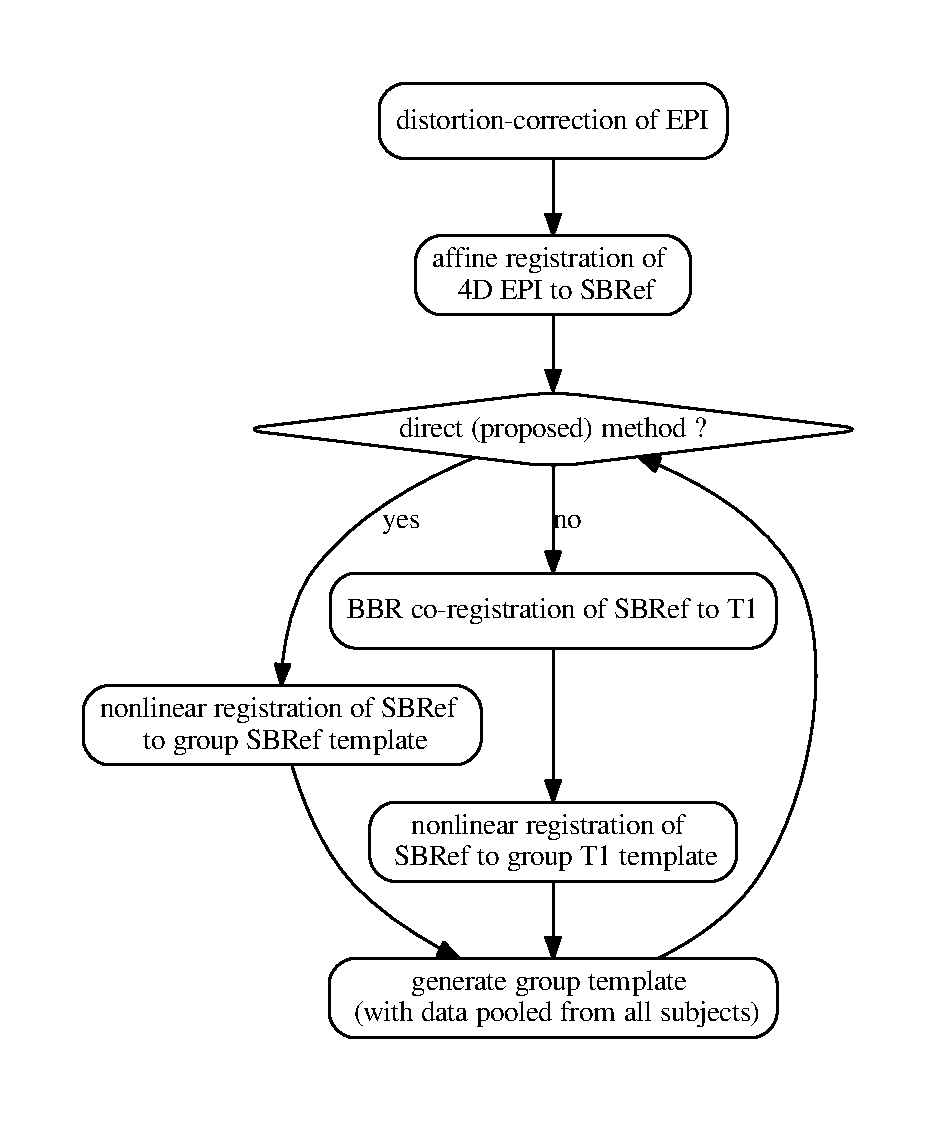
\includegraphics[width=1\linewidth]{flowchart.pdf}
\caption{\textbf{The pipelines.} The template-generation step is done using ANTs~\citep{avants2008,avants2011}. It pools registered data from all subjects. \textbf{N.B.:} SBRef = single-band high-resolution 3D volume. As in \citep{glasser2013}, all the transformations are postponed and the original 4D EPI is resampled at the end by applying the composition of these transformations in a single step.}
\label{fig:pipelines}
\end{figure}

\paragraph{Deformation model}
We used ANTs' \textit{Symmetric Normalization} (aka \textit{SyN})
deformation model ~\citep{avants2008,avants2011}, which has been shown
to be a state-of-the art method for nonlinear registration
\citep{pmid19195496}. As done usually, we initialize a nonlinear
registration algorithm with an affine (rigid-body) registration
algorithm.
%
The former is simply meant to estimate an alignment for the
bounding boxes of the images (thus ensuring a sufficiently large
region of overlap). Concretely, we stack a 2-level
pyramidal\footnote{\textit{Pyramidal} means multiple passes are
made by a registration algorithm on the input images, with finer
and finer resolution (aka \textit{pyramid}). In this speedup technique, each
pass of the pyramid is initialized with the solution of the
previous pass (this is known as \textit{warmstarting}).}  affine
transformation model (as initialization) with a 3-level pyramidal
SyN deformation model. \textit{Mattes mutual information}
\citep{mattes2003} is used as the loss function.

%% This model is triggered in ANTs \citep{avants2008,avants2011} using the following command-line options:
%% \begin{verbatim}
%% 	    --transform Affine[ 2.0 ]
%% 	    --metric Mattes[ ${fixed_img}.nii.gz, ${moving_img}.nii.gz, \
%%               1, 32, Random, 0.05 ]
%% 	    --convergence [ 1500x200, 1e-08, 20 ] --smoothing-sigmas \
%%               1.0x0.0vox
%% 	    --shrink-factors 2x1 --use-estimate-learning-rate-once 1
%% 	    --use-histogram-matching 1
%% \end{verbatim}

\subsection{The pipelines}
\label{sec:pipelines}
%% In the sequel, we will use the following acronyms to describe the
%% different pipelines: ``\textit{single-band highres}'': means the
%% pipeline uses the single-band high-resolution EPI volume.
We now present constructions for the pipelines whose benchmark is the
core of this work. All registration pipelines presented here were
scripted in using command-line tools from FSL version 5.0
\citep{smith2004} for affine registration, distortion correction,
motion correction, ANTs \citep{avants2009advanced}
antsRegistration, antsApplyTranforms, and some custom scripts
(for distortion correction) from the HCP scripts described in
\citep{glasser2013}, hosted on Github.
Except stated otherwise, all affine registrations (motion correction,
coregistration) were performed using FSL's \textit{flirt} tool
\citep{smith2004} with Normalized Mutual Information as cost the function (option: \textit{-cost
  normmi}).

\subsubsection{Classical indirect T1-based method}
\label{sec:classical}
The classical indirect T1-based pipeline for registration of EPI images can be schematized as
follows\footnote{The ``$\circ$'' symbol denotes composition of transformations.}:
\begin{eqnarray}
  \begin{split}
    \hspace{-1.8em}\text{EPI} \rightarrow \text{templ.} =
    \underbrace{(\text{T1} \rightarrow \text{templ.})}_{\text{nonlinear}} \circ \underbrace{(\text{EPI}_0
      \overset{\text{BBR}}{\rightarrow} \text{T1})}_{\text{linear}} \circ \text{DistCorr}
    \end{split}
  \label{eq:dct1_pl}
\end{eqnarray}
in which a deformation of the subject's T1 is
estimated and this deformation is then used to warp the same subject's
EPI data. We implemented the pipeline as follows. Here, $\text{EPI}_0$ is any single-volume EPI
image previously-coregistered with the 4D EPI sequence. Typical choices include: the middle
volume of the film or the mean volume after motion correction. In our implementations, we used the
former.

 For the template, a subject is fixed
and its T1 image is used as the template. For each other subject,
\textit{(a)} distortion correction is used to learn a nonlinear
    undistorting warpfield, in a procedure already described in
    subsection \ref{sec:gen_proc} above. Then,
\textit{(b)} motion correction is done to realign the the
subject's EPI data to the mean thereof.
    The subject's T1 image is then aligned to this
    mean EPI image via coregistration (an affine transformation).
We use BBR (boundary-based registration)
    \citep{greve2009accurate} for this coregistration step,
    for optimal results and fair comparison.
    BBR is a state-of-the-art functional-to-structural registration method driven by intensity
    difference across boundary (samples). It uses white-matter boundaries (via T1w segmentation).
    BBR need good structural images
    (with little contrast bias), and some anatomical contrast in the EPI image (which
    is the case of the single-band high-resolution reference images in the HCP dataset
    \citep{VanEssen20122222}). The implementation we use is \textit{epi\_reg} script of FSL
    \citep{smith2004}.
    However, since BBR is an affine correction method, it still suffers from the limitations explained in
    the introductory section. In particular, it is not resiliant to distortions in the input EPI
    image.
    
    % This method is supposed to be more robust to pathologies and artefacts in EPI

\textit{(c)} ANTs is used to learn a deformation of the T1
    image to the
    template (which is a fixed subject). This produces a warped
    version of the T1 image, together with the corresponding
    deformation (and its inverse too), for passing from the subject's
    space to the template space. Finally,
\textit{(d)} the deformation above (T1-based), and all the
    other postponed
    warpfields, affine transformations, etc., are then applied (in
    respective order) to all EPI data previously aligned (rigidly, via
    coregistration) with the T1 image of the subject; these may
    include EPI images acquired on the same subject during another task,
    for instance. This one-step resampling procedure (see subsection
    \ref{sec:gen_proc}) then produces a registered, motion-corrected,
    undistorted version of the input EPI data.
\label{sec:classical}

Then mean of all the registered T1 images is computed, and becomes the template henceforth. This procedure is iterated a couple of times.

%% \paragraph{A note on BBR}
%% \begin{itemize}
%% \item EPI to structural registration \citep{greve2009accurate}. See Fig. \ref{fig:bbr}.
%%   \begin{itemize}
%%   \item incorporates fieldmap correction (previously FUGUE)
%%   \item used in FEAT (B0 unwarping)
%%     \end{itemize}
%% \item Uses white-matter boundaries (via T1w segmentation)
%%   \begin{itemize}
%% \item Need good structurals (not too much bias field)
%% \item However, also requires anatomical contrast in the EPI!
%% \item Driven by intensity difference across boundary (samples)
%%   \end{itemize}
%% \item More robust to pathologies and artefacts in EPI
%% \end{itemize}


%% \begin{figure}[!h]
%%   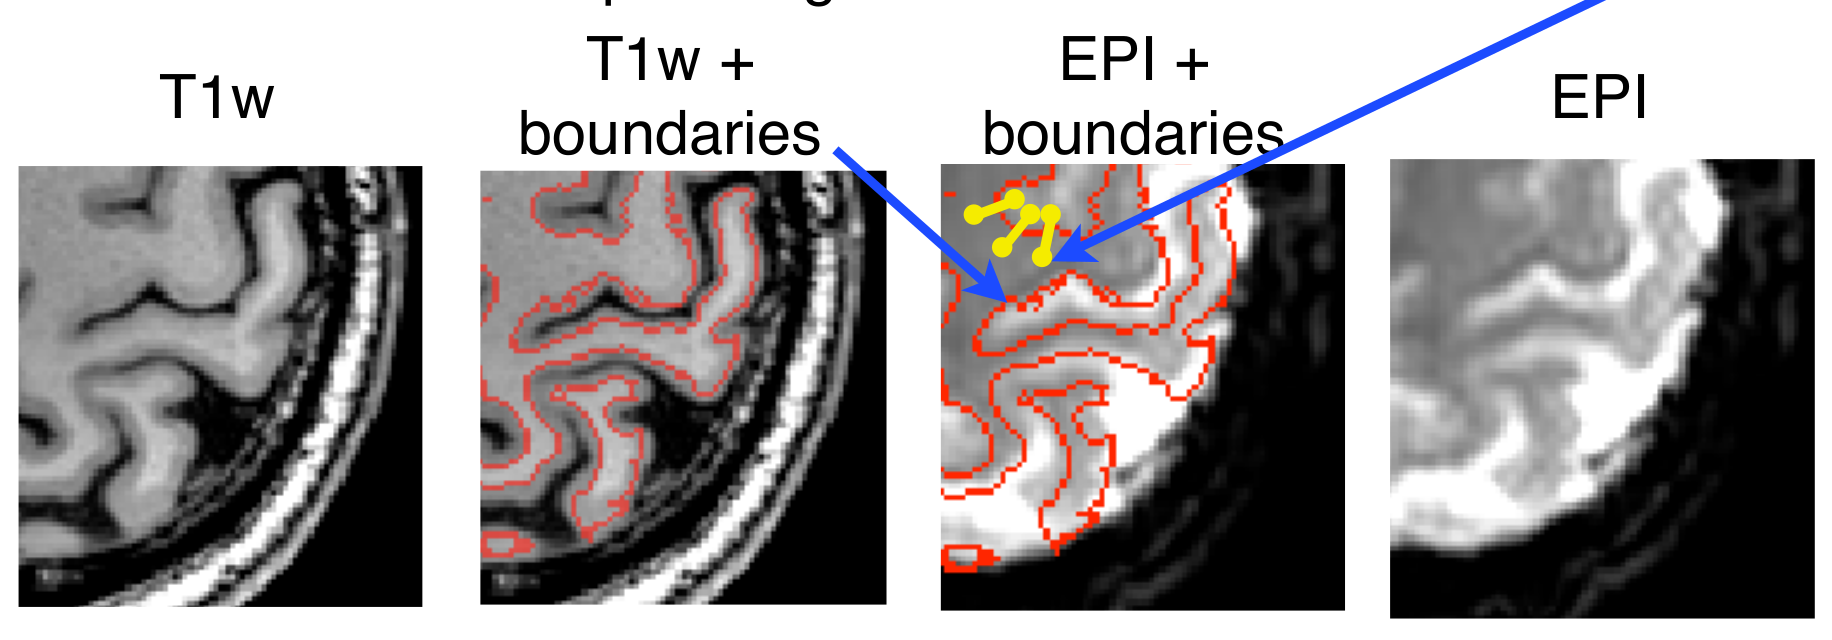
\includegraphics[width=1\linewidth]{figs/bbr.png}
%%   \caption{\textbf{XXX: Supplements notes on BBR. Figure borrowed from FSL course without permission.
%%       We need to generate ours!!!}}
%%   \label{fig:bbr}
%% \end{figure}

\subsubsection{Our proposed \textit{direct} EPI-based non-linear  inter-subject
  registration method}
\label{sec:proposed}
Our proposed pipeline operates just as the
classical indirect T1-based pipeline described above in
\ref{sec:classical}, except that the anatomical image is replaced with
the single-band high-resolution EPI (the SBRef) image, which has more tissue contrast than the any volume of the 4D EPI film being registered
\citep{glasser2013}, and also does not suffer from multi-band artifacts. The anatomical image is not used anywhere in
this pipeline.  The pipeline can be schematized as follows:

\begin{eqnarray}
  \begin{split}
    \text{EPI} &\rightarrow \text{templ.}
    = \underbrace{(\text{EPI}_0 \rightarrow \text{templ.})}_{\text{nonlinear}} \circ  \text{DistCorr},
    \label{eq:dcsbref_pl}
    \end{split}
\end{eqnarray}
where we take $\text{EPI}_0 = $ Single-band high-resolution (SBRef) EPI image.
%% We implemented and experimented both of these variants of our method
%% and benchmarked them against the classical technique presented in
%% \ref{sec:classical} above.

\paragraph{A note on image interpolation (resampling)}
To avoid degrading the images as they travel through a pipeline, we
stack all intermediate transformations and postpone the resampling
operations to the end of the pipeline. The transformations are then
concatenated (i.e composed), and applied to the input image in a
one-step resampling procedure based on the \textit{ApplyTransforms}
tool of the ANTs software \citep{avants2008,avants2009advanced}. For
example,  affine transformations estimated during the
motion correction step are converted to warpfields using FSL's
\textit{convertwarp} tool \citep{smith2004}. FSL's \textit{applywarp}
tool \citep{smith2004} is then used to jointly apply this affine
transformation warpfields and the warpfields corresponding to the
deformations estimated by \textit{topup} \citep{smith2004}, which
are then stacked with subsequent transformations. We use this strategy in both pipelines.

\section{Relation to previous  works}
\subsection{Direct EPI-to-EPI non-linear inter-subject  registration}
% It should be noted that
The idea of EPI-to-EPI registration has already been suggested in the
literature. For example, the method in \citep{grabner2014} used
high-resolution EPI (1.1mm isotropic) data for different subjects
acquired at 7T to iteratively build a sequence of EPI-based
study-specific templates of increasing quality / resolution
\citep{pmid17354756}. The finest of these templates shows a great deal
of anatomical detail. Group-level activation patterns for a
finger-tapping task were also shown to be very accurately localized on
the posterior bank of the central sulcus. The authors concluded that
high-resolution (7T) EPI images contain enough anatomical information
for inter-subject registration, and so one can effectively by-pass the
anatomical image of subjects in pipeline. This would for example allow
one to avoid the classical coregistration step used to align the
subject's EPI images to their anatomy.  Our experiments confirm and
extend the findings of \citep{grabner2014}, but at an even lower
resolution: 2mm resolution, obtained from 3T MRI, and on a much larger
dataset. Indeed, using a much larger bail of 110 subjects, from Human
Connectom Project (HCP) dataset \citep{VanEssen20122222}, and a variety
of different task contrasts, we show that registration with our
pipeline increases the pairwise NMI of subjects, over the classical
pipeline; crucially, this leads to a decrease in residual
post-registration inter-subject misalignement.

%% We observe however that our EPI-based pipeline leads group-level GLM results
%% which are comparable to results using the classical T1-based
%% registration pipelines. 
%% %
%% The fact that these statistical estimation procedures (GLM, ICA, etc.)
%% are insensitive to improvements in inter-subject registration implies
%% that inter-subject variability is dominated by other factors: the
%% variability of the size of the effects and their exact anatomical
%% localization, beyond the variability of  brain shapes.

In comparison, the pipeline we propose (refer to \ref{sec:proposed})
is much lighter computationally as
we bypass the potentially expensive and challenging step of generating a good
template from EPI data \citep{pmid17354756}. Of course, this economy is
more of a compromise between complexity and accuracy, and might be potential
limitation of our
contribution.  Finally, we note that the work in \citep{grabner2014}
did not consider the distortion problem which are severe even at 3T
\citep{anderson2003}, as it is the case with the HCP data.

\subsection{Non-linear EPI-to-structural coregistration}
A recent work \citep{wang2017} has considered the possibility of replacing the classical
linear EPI-to-structural coregistration step with a non-linear counterpart,
and then running a non-linear structural-to-template registration as usual.
They show that their method outperforms the method based on distortion correction
and linear EPI-to-structural coregistration followed by structural-to-template
registration as usual (see \ref{sec:classical}). In contrast, our proposed
method (refer to \ref{sec:proposed}) does not use the structural image at all.


\section{Experiments}
\label{sec:exp_epi2epi}
We now describe benchmarks done to compare the pipelines presented in
this paper (subsection \ref{sec:pipelines}) on the task fMRI data of
110 subjects from the HCP dataset \citep{VanEssen20122222}. 
The task fMRI data were acquired in an attempt to assess major domains
that
% are thought to
sample the diversity of neural systems, including: 1) visual, motion,
somatosensory, and motor systems; 2) language processing (semantic and
phonological processing); 3) social cognition (Theory of Mind); and 4)
emotion processing.
Due to time constraints, our benchmarks were run only on these 4 (out
of a total of 7) tasks (i.e protocols). Also, only data for LR (left-right)
phase-encoding direction \citep{chang1992technique} runs were used. In all the non T1-based
pipelines, the single-band high-resolution (SBRef) image of the motor
task was used to learn deformations of the subject's brain into
template space (a fixed subject of the same dataset).

The estimated
deformations were then applied to warp EPI data (previously
coregistered to same subject's motor SBRef) acquired on the same
subject during different task conditions, into template space.
GLMs (General Linear Models) \citep{friston1994statistical} were run
using \textit{nipy} \citep{Gorgolewski2011}, open-source Python library for analysis of neuro-imaging data. For the purpose of reporting the results, the resulting maps were was co-registered to
MNI space a posteriori.

\subsection{Evaluation metrics}
The pipelines were evaluated using the following qualitative and quantitative
metrics.

%% \textbf{Here you really need to state :
%% * What your hypotheses are; how you check them
%% * what experiments you're going to carry out
%% * what your evaluation metrics are}.

\subsubsection{Normalized mutual information evaluation (NMI)}
NMI (see section \ref{sec:notations} for definition) is a
popular similarity metric used to assess the quality of
registration between two images, i.e how well aligned the images are to one another
(for example \citep{maes1997multimodality}). It is also the loss function minimized by many
optimization algorithms in image registration.
A detailed overview of
the use of the NMI metric in medical image registration can be found
in \citep{pluim2003}.
In our experiments, FSL's \textit{flirt} \footnote{With the
   ``\textit{-schedule}'' option.}
tool \citep{smith2004} was used to compute NMI. 

%%  In the
%% supplementary materials,
%% we have provided for each pipeline, an animated GIF file of the
%% concatenated registered EPI images. These GIF movies highlight
%% significant difference between the indirect and direct registration
%% models, differences which are in accordance with the statistical
%% results presented here.

\subsubsection{Inter-subject residual variance}
In a good registration method, the residual subject-to-subject
variance of the EPI image should be reduced. The aim of
inter-subject registration is indeed to put subjects into spatial
correspondence to facilitate later group analysis. To measure the quality of
the different registration methods in this regards, we computed the
coefficient of variation (CoV) across the different subjects after registration.
This is defined by

\begin{equation}
  \text{CoV} = \frac{\text{variance image across subjects}}{\text{mean image across subjects}}.
\end{equation}

High values in this 3D image would outline regions of the brain which are not well registered across subjects.

% \textbf{XXX Mention that you used CoV and give the corresponding formula.}

%% \begin{figure*}[!htbp]
%% \includegraphics[width=.161\linewidth]{figs/LH-RH_DC+T1.png}
%% \includegraphics[width=.161\linewidth]{figs/LH-RH_DC+SBRef.png}
%% \includegraphics[width=.161\linewidth]{figs/LF-RF_DC+T1.png}
%% \includegraphics[width=.161\linewidth]{figs/LF-RF_DC+SBRef.png}
%% \includegraphics[width=.161\linewidth]{figs/FACES-SHAPES_DC+T1.png}
%% \includegraphics[width=.161\linewidth]{figs/FACES-SHAPES_DC+SBRef.png}
%% \includegraphics[width=.32\linewidth]{figs/LH-RH_blobs.png}
%% \includegraphics[width=.32\linewidth]{figs/LF-RF_blobs.png}
%% \includegraphics[width=.32\linewidth]{figs/FACES-SHAPES_blobs.png}
%% %% 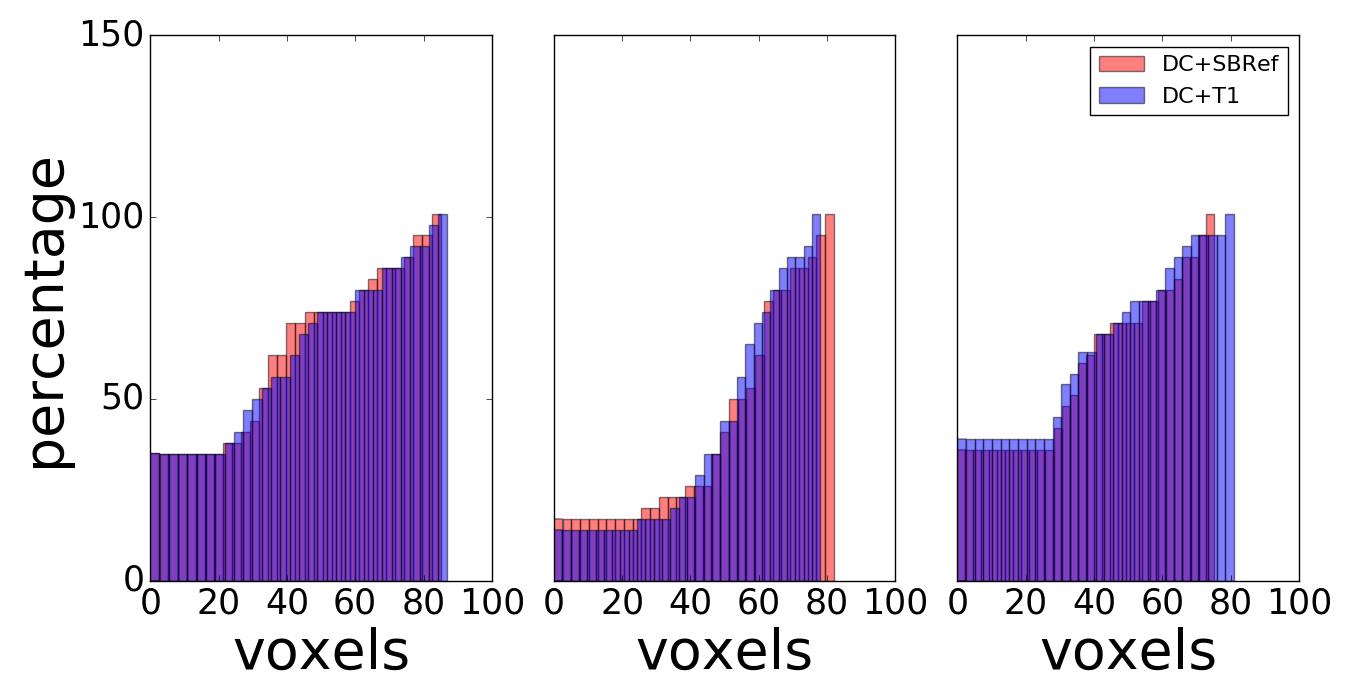
\includegraphics[width=.32\linewidth]{figs/LH-RH_hist.png}
%% %% 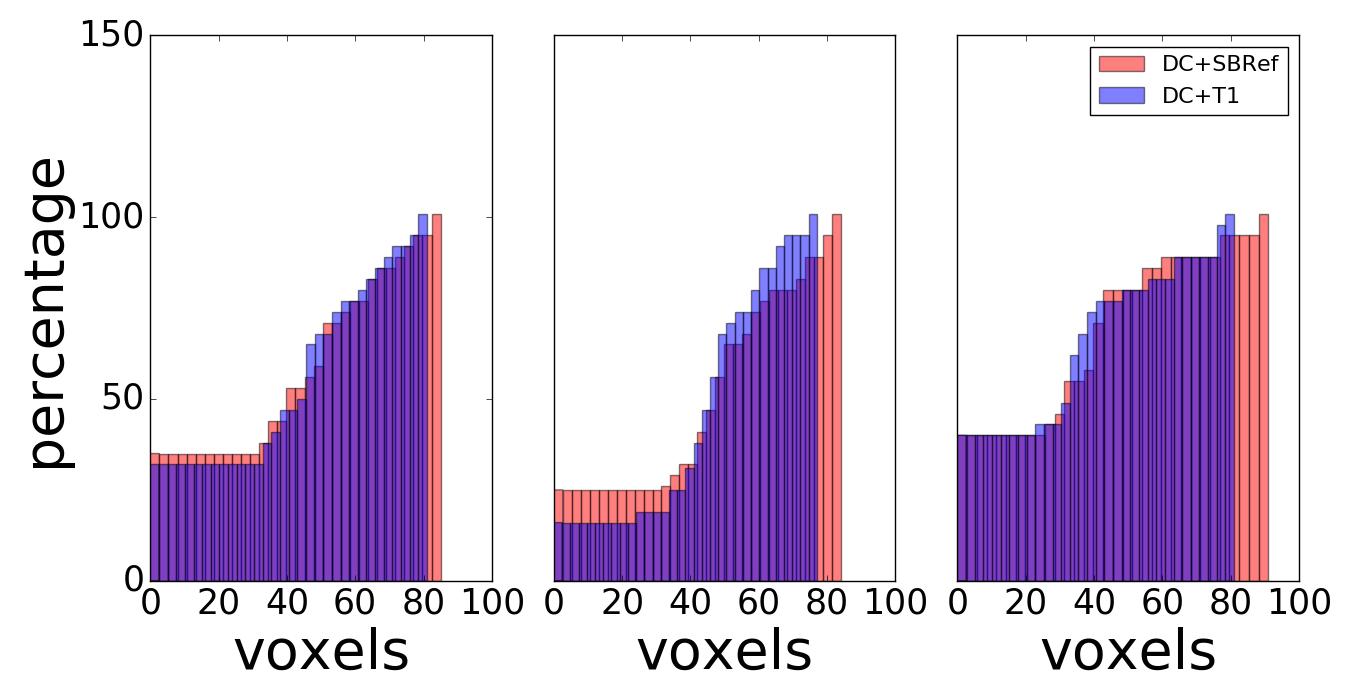
\includegraphics[width=.32\linewidth]{figs/LF-RF_hist.png}
%% %% 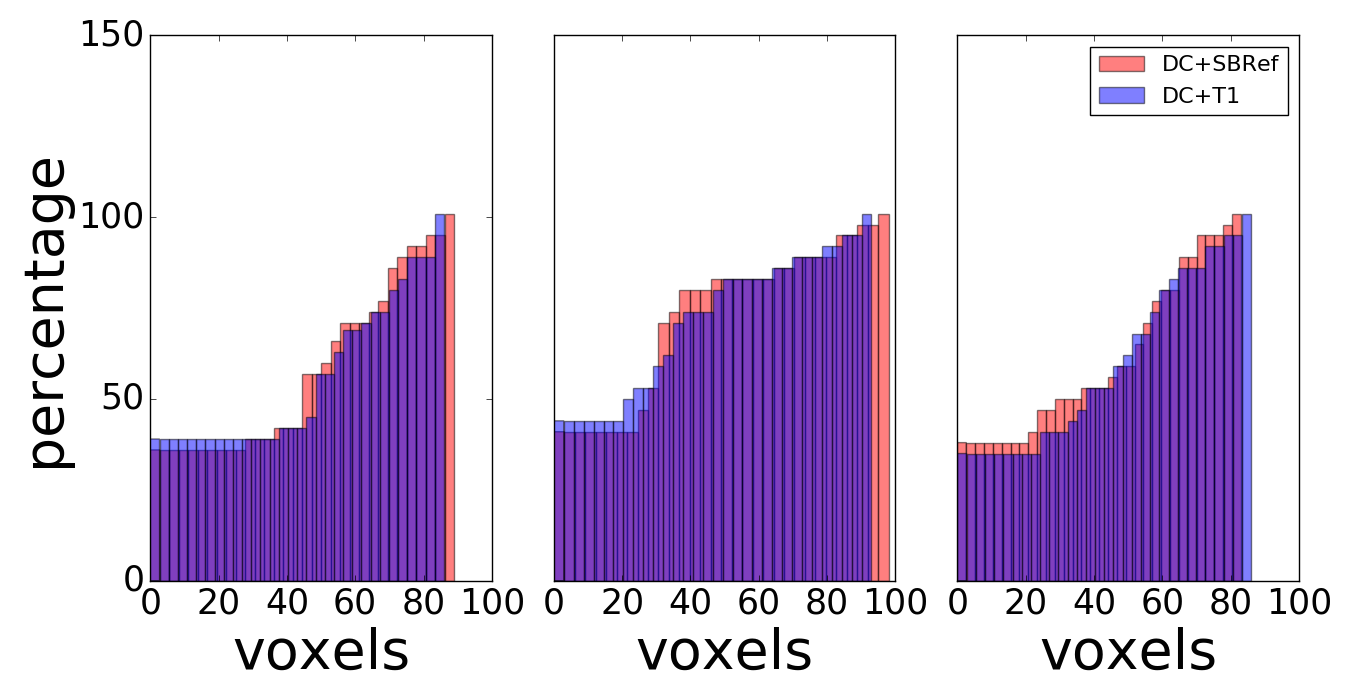
\includegraphics[width=.32\linewidth]{figs/FACES-SHAPES_hist.png}

%% 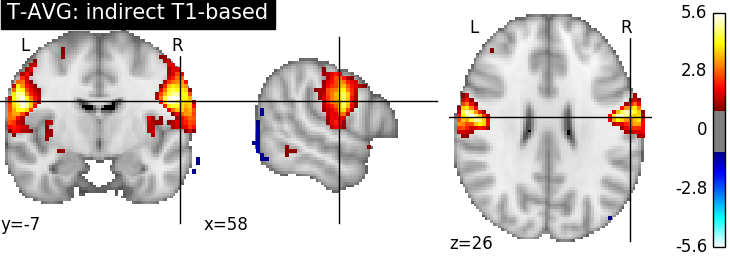
\includegraphics[width=.161\linewidth]{figs/T-AVG_DC+T1.png}
%% 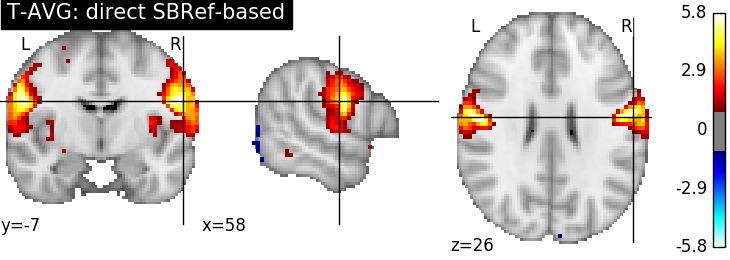
\includegraphics[width=.161\linewidth]{figs/T-AVG_DC+SBRef.png}
%% %% \includegraphics[width=.161\linewidth]{figs/0BK-2BK_DC+T1.png}
%% %% \includegraphics[width=.161\linewidth]{figs/0BK-2BK_DC+SBRef.png}
%% 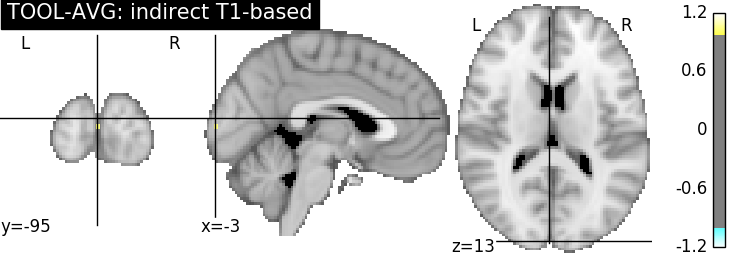
\includegraphics[width=.161\linewidth]{figs/TOOL-AVG_DC+T1.png}
%% 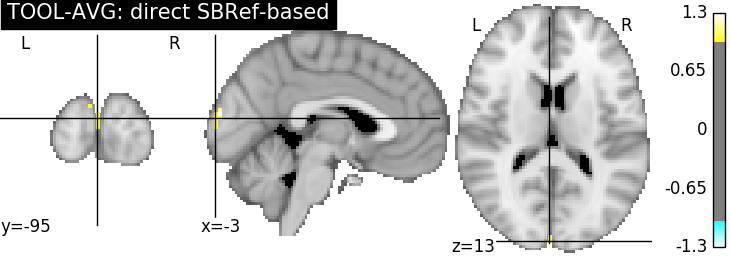
\includegraphics[width=.161\linewidth]{figs/TOOL-AVG_DC+SBRef.png}
%% 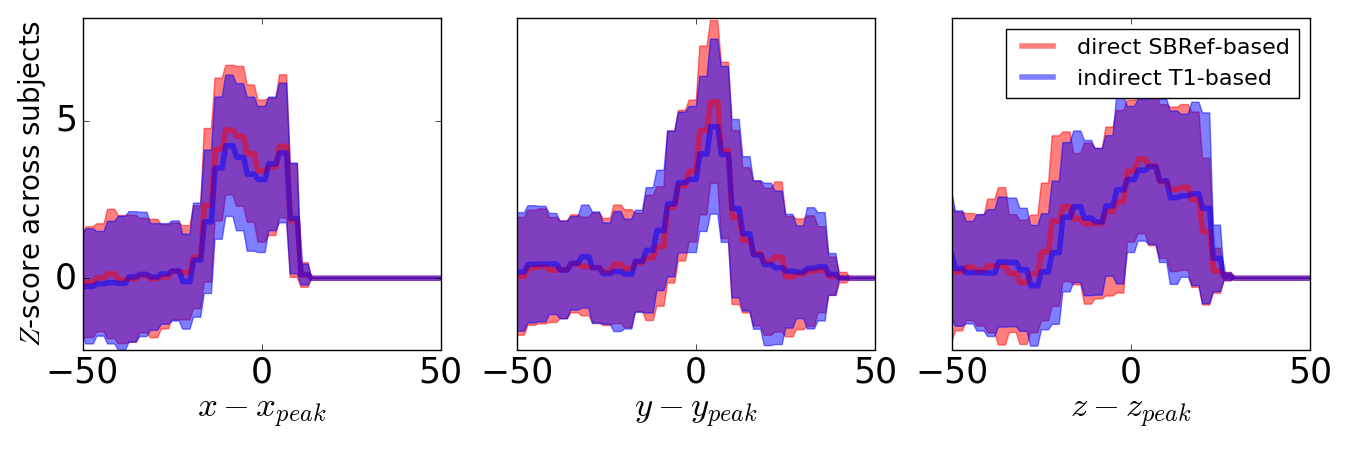
\includegraphics[width=.32\linewidth]{figs/T-AVG_blobs.png}
%% 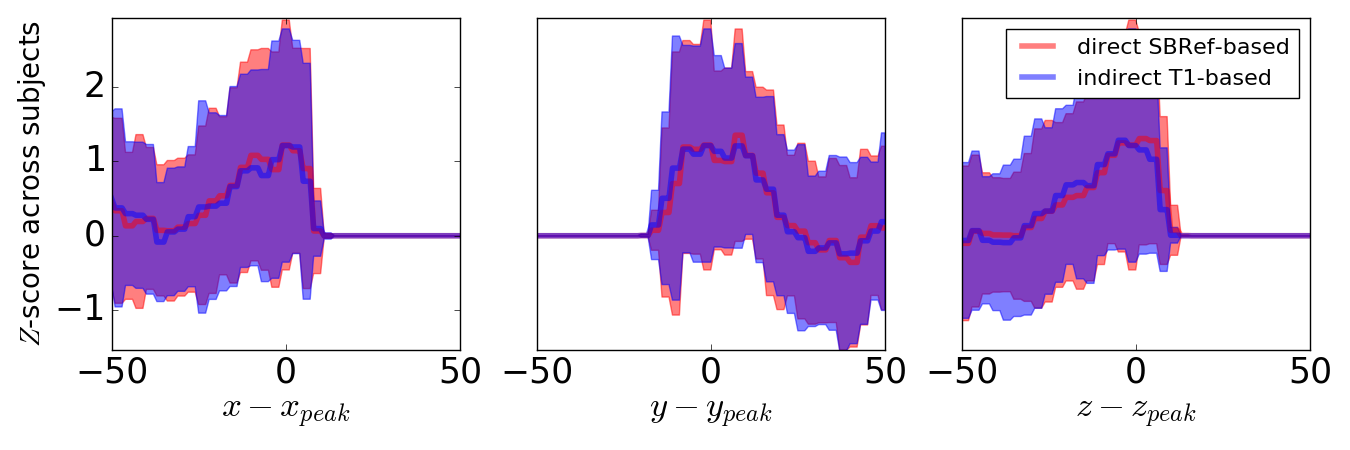
\includegraphics[width=.32\linewidth]{figs/0BK-2BK_blobs.png}
%% 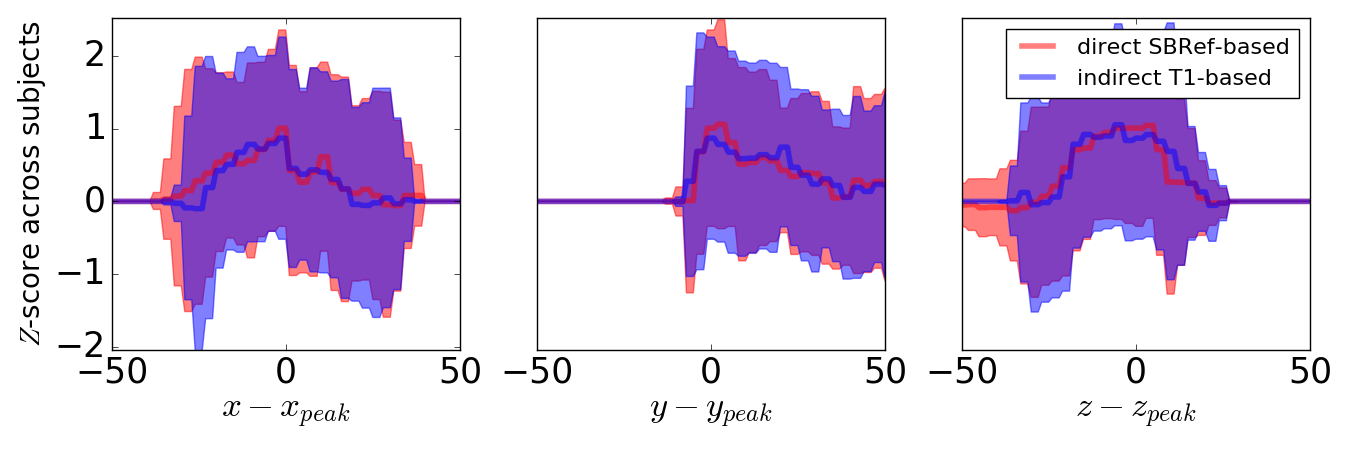
\includegraphics[width=.32\linewidth]{figs/TOOL-AVG_blobs.png}
%% %% 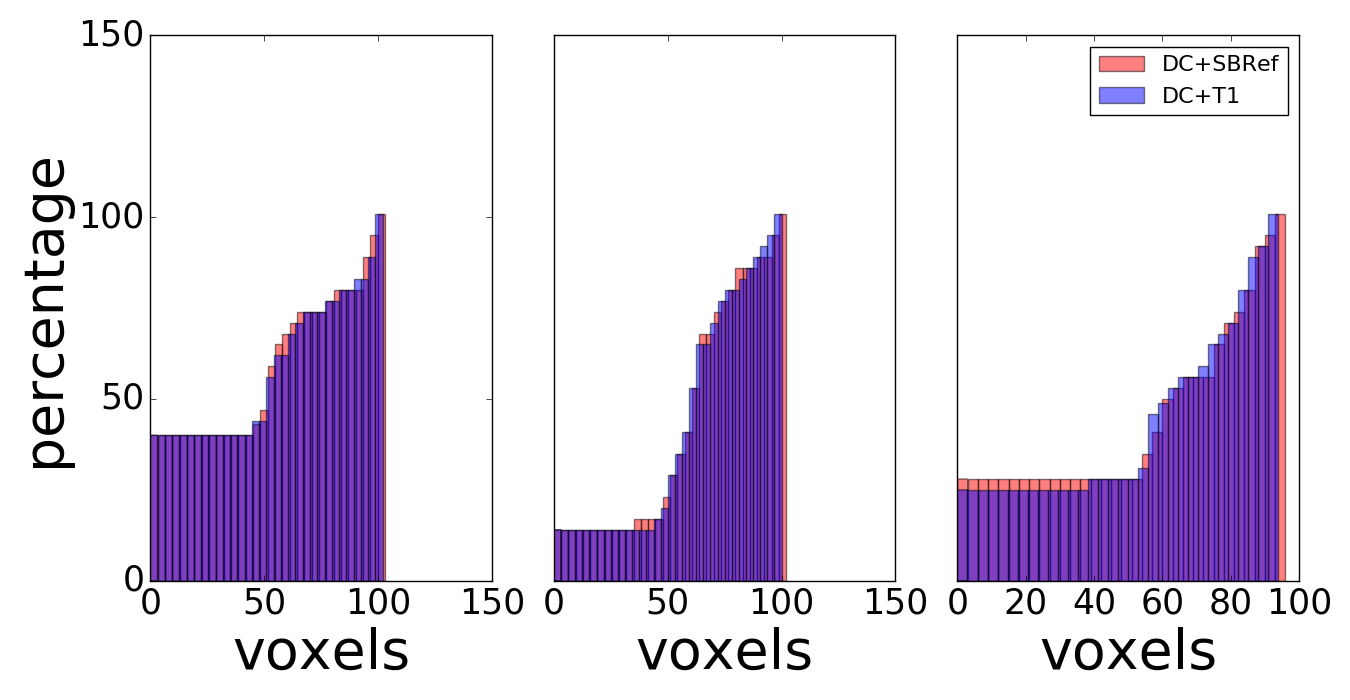
\includegraphics[width=.32\linewidth]{figs/T-AVG_hist.png}
%% %% 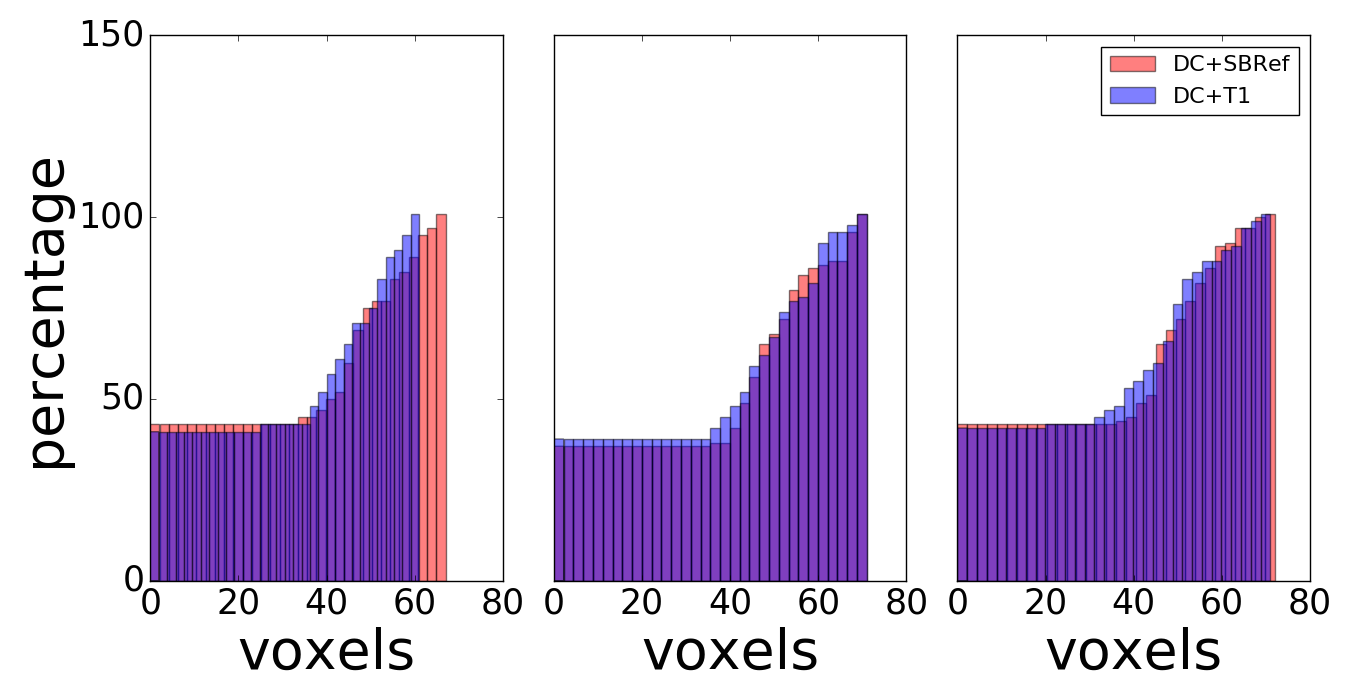
\includegraphics[width=.32\linewidth]{figs/0BK-2BK_hist.png}
%% %% 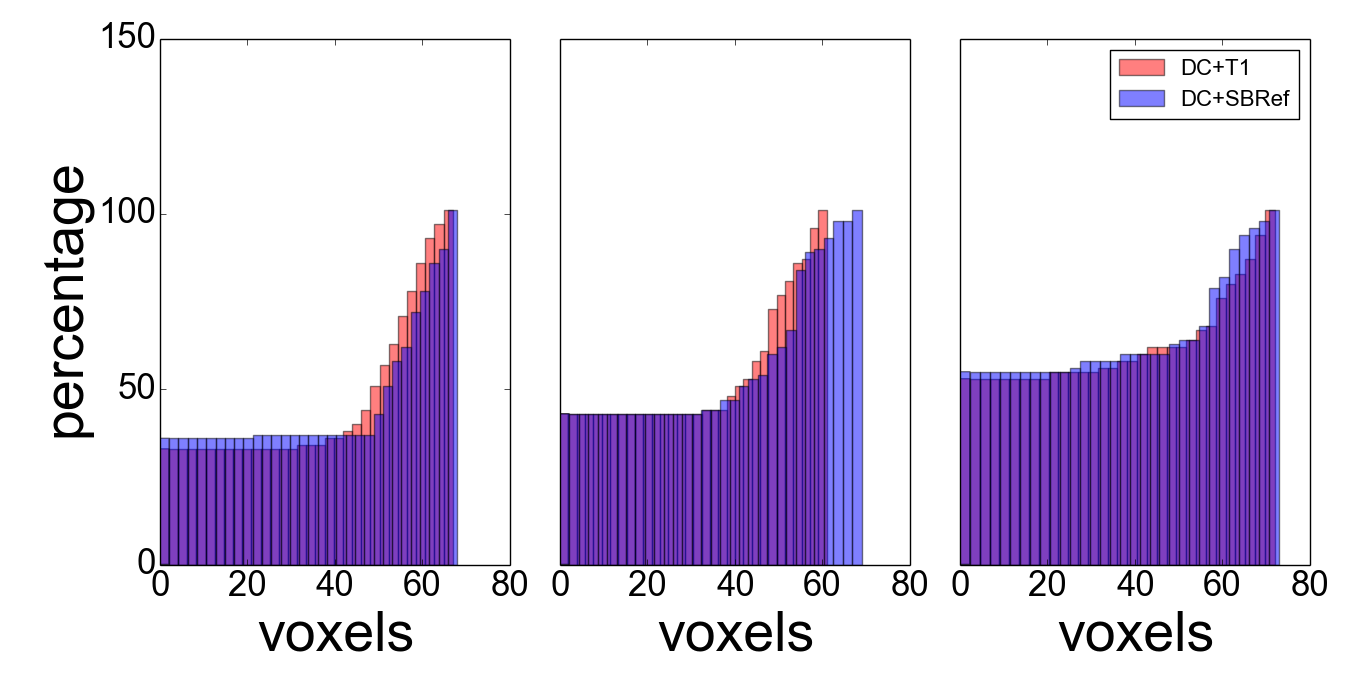
\includegraphics[width=.32\linewidth]{figs/TOOL-AVG_hist.png}
%% \caption{
%%   Thresholded images GLM $Z$-scores for
%%  different task contrasts (LH-RH, FACES-SHAPES, etc.) averaged
%%  across subjects...}
%% \end{figure*}

\subsubsection{Group-level statistics and functional brain network patterns}
Finally, in a successful inter-subject registration procedure, we
expect the functional activation patterns to more localized in space
and to have higher peaks. Or could this effect could be
masked by inter-subject variability in activation magnitude ?
This will be discussed in detail in the discussion section \ref{sec:discussion}.

\subsection{How many (plausible) pipelines are there ?}
It is worth noting that potentially hundreds of pipelines which could
have considered for testing: should we do distortion correction ? And
if yes, how ? Should we use linear or nonlinear model for the
deformation field ?
%
What degree should we use for the interpolating splines ? In fact as
noted in \citep{Poldrack059188}, there are exponentially many pipelines
that can be considered, based on the answers to the above choices.
%
Of course some of these parameters have rule-of-thumb default values
(for example, there is no doubt distortion correction is a good thing
to do), but others are open to preferential choice. Thus our goal is
not to consider all possible pipelines, but to look at a more focal
question: does direct EPI-based inter-registration outperform the
traditional indirect T1-based pipeline ?


\section{Results}
\label{sec:results}
We now present results of experiments performed on the task fMRI
protocols of the HCP dataset \citep{VanEssen20122222}. Refer to
section \ref{sec:exp_epi2epi} for detailed information about the
experiments we did. The different pipelines discussed in section
\ref{sec:pipelines} were used to register the data (inter-subject
registration), and the quality of the registration was benchmarked
using the different evaluation metrics discussed in Section \ref{sec:exp_epi2epi}. 

\subsubsection{Normalized Mutual Information (NMI)}
The results comparing across-subject NMI for the pipelines are presented in Figure \ref{fig:nmi}. We see that MNI is in most cases higher through our approach, which implies that 
our proposed direct EPI-based pipeline mildly outperforms the classical indirect T1-based pipeline.

\begin{figure}[!htbp]
  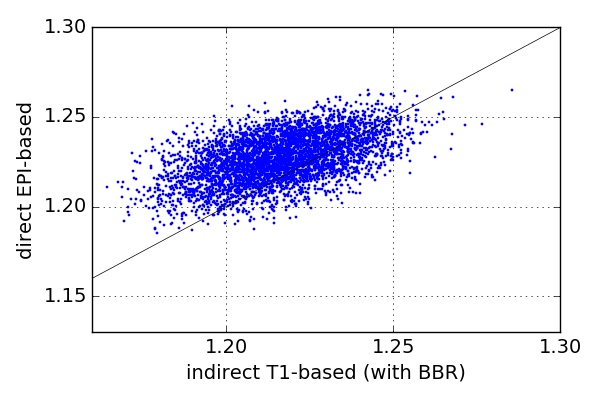
\includegraphics[width=1\linewidth]{figures/nmi_new_DC+T1_new_DC+SBRef.png}
  % 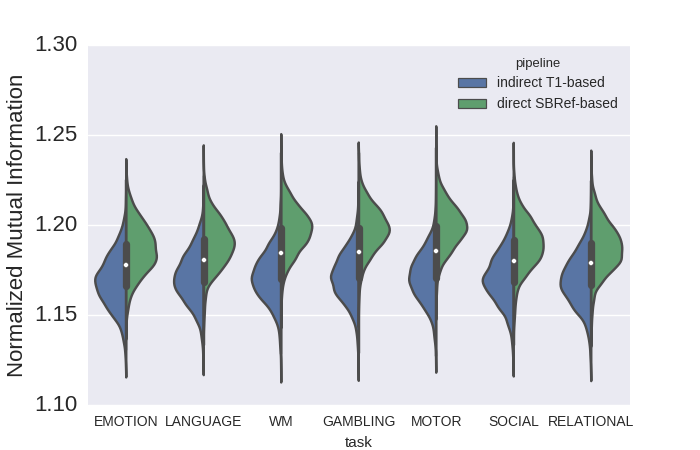
\includegraphics[width=1\linewidth]{figures/nmi_violin1.png}
\caption{Normalized Mutual Information -- NMI (higher values are
  better). % \textbf{Top:}
  %% Each color represents date from an HCP task.
  Each point
    $(x, y)$ on the
    plots such that $x$ is the NMI of a given pair of subjects
    registered using the pipeline on
    the abscissa and $y$ is the NMI of the same pair of subjects
    registered using the pipeline on the ordinate.
    % Different colors represent different tasks (i.e functional protocols).
    From the one-sided
    %% Wilcoxon rank-sum statistics ($W$) testing the one-sided
    %% hypothesis $\mathcal{H}: X \le Y$, where $(X, Y)$ is the (unknown)
    %% random vector of which each sample point $(x, y)$ is a realization.
    %% See figure legends for the numerical values and significance of
    %% the statistics.
    We see that our proposed direct EPI-based pipeline
    significantly outperforms the classical indirect T1-based
    pipeline.
    %% \textbf{Bottom:} Violin-plots of the same the same information as in
    %% the \textbf{Top} plot, presenting another view of the results.
    %% pipeline, indicating that EPI-to-EPI inter-subject registration is
    %% better than the classical indirect T1-based technique.
}
\label{fig:nmi}
\end{figure}

%% \begin{figure}
%% 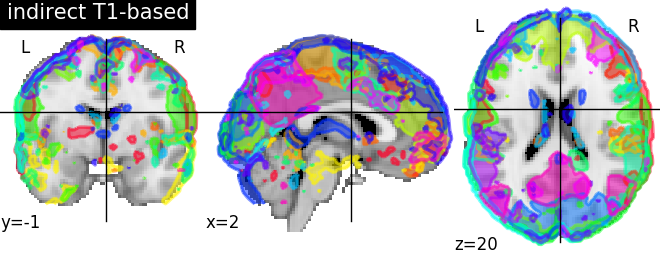
\includegraphics[width=1\linewidth]{figures/DC+T1_ica_atlas.png}
%% 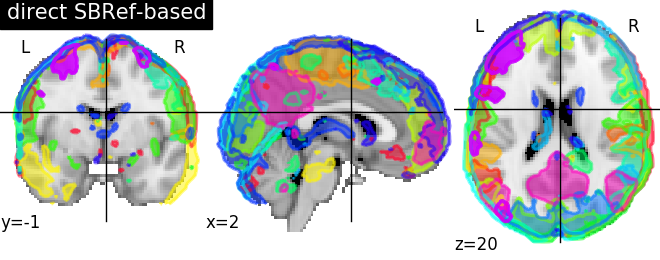
\includegraphics[width=1\linewidth]{figures/DC+SBRef_ica_atlas.png}
%% \caption{Atlas of 16 network patterns from Independent
%%   Component Analysis (ICA). Maps obtained using the \textit{nilearn}
%%   \citep{abraham2014machine} implementation of CanICA\citep{varoquaux2010group,varoquaux2010ica} after inter-subject registration, on multi-subject functional data
%%   registered using the different pipelines. We see that the geometry of the patterns are essentially the same across the different pipelines. The Default Mode Network \citep{raichle2001} has been labeled pink; a more detailed view of this network is presented in Figure \ref{fig:dmn} of the supplementary materials section.}
%%   \label{fig:atlas}
%% \end{figure}


\subsubsection{Residual inter-subject spatial variability}
\begin{figure}[!htb]
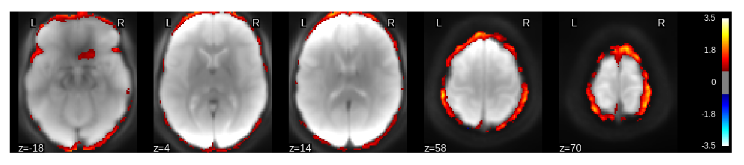
\includegraphics[width=1\linewidth]{figures/cov1.png}
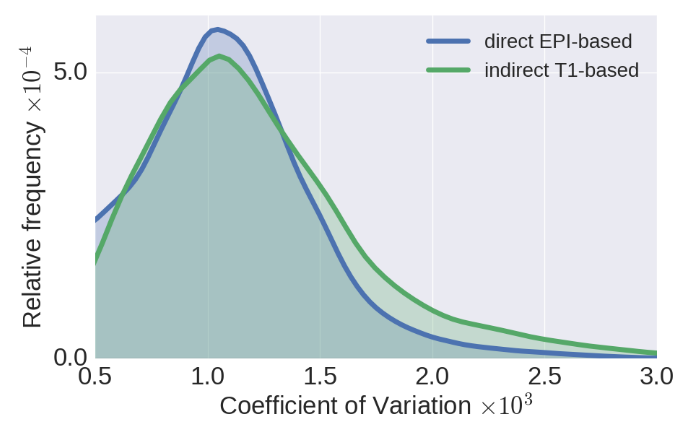
\includegraphics[width=1\linewidth]{figures/cov2.png}
\caption{\textbf{Coefficient-of-Variation (CoV)} after registration. \textbf{Top:} Log10 of ratio of across-subject Coefficient of Variation (CoV) for indirect T1-based pipeline / direct EPI-based. We see that the gain of our proposed method is most pronounced along the cortical surface.
\textbf{Bottom:} Histograms of CoV  for both
  pipelines. Again, we see clearly that our proposed method reduces the inter-subject variability by a much larger margin, indicative of improved subject-to-subject alignment.}
\label{fig:cv}
\end{figure}

In Figure \ref{fig:cv}, we show across-subject histograms of
across-subject per-voxel Coefficient of Variation (small is better).
We see that our proposed direct method outperforms the classical indirect T1-based method, as the former leads to relatively more mis-aligned voxels across subjects, most concentrated on the outer edge of the cortex (see Figure \ref{fig:cv} \textit{(a)}).

\subsubsection{Quality of estimated EPI group template}
To compare the quality of the group template produced by either pipeline, a snapshot of the resulting mean image or template is displayed in
Figure \ref{fig:template}. Compared to the our proposed direct method,
the mean image (across all subjects) from the indirect T1-based
pipeline is blurry and has ``ripples'' on the cortical surface,
indicative of residual mismatch between subjects after
registration. The across-subject mean image post-registration with our
direct EPI-based pipeline is the sharpest, showing that the subjects
have been matched extremely well. Also, one notices that the mean image from
the indirect T1-based pipeline still has some residual distortion (here in the
left-to-right direction), even though distortion correction was done as part of both pipelines.

\begin{figure}[!htbp]
  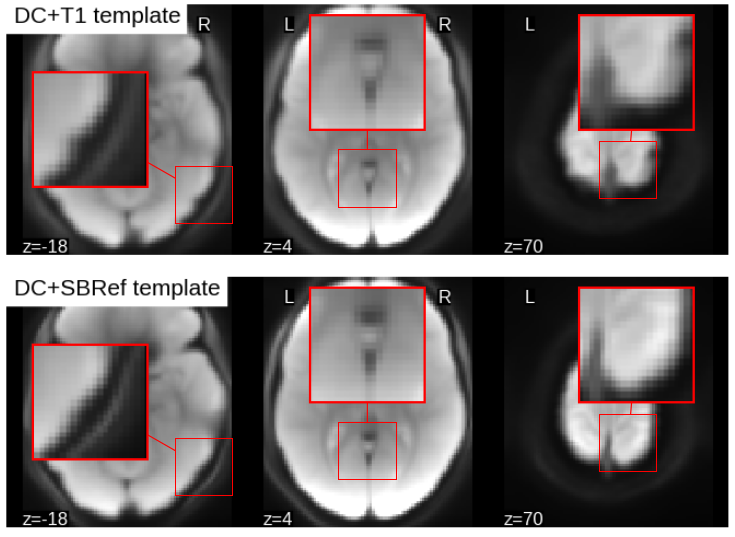
\includegraphics[width=1\linewidth]{figures/template.png}
\caption{Mean EPI image
  across all subjects after registration (aka estimated population
  templates). Patches on the images have been zoomed to highlight
  details. The mean image from the indirect T1-based
  pipeline (\textbf{Left}) is more blurry (as seen here in the
  cerebellum), compared to
  our direct EPI-based pipeline post-registration across-subject mean
  image (\textbf{Right}) which is much sharper, indicative of a
  better inter-subject
  registration. Also the mean image from the T1-based pipeline has
  ripples on the cortical surface indicative of residual registration
  problems, which can be attributed residual EPI-distortions that
  could not be captured via coregistration.}
\label{fig:template}
\end{figure}



\subsubsection{Group-level statistics and Functional brain network patterns}
\begin{figure}[!htbp]
%% \includegraphics[width=.48\linewidth]{figures/0BK-2BK_DC+T1.png}
%% \includegraphics[width=.48\linewidth]{figures/0BK-2BK_DC+SBRef.png}
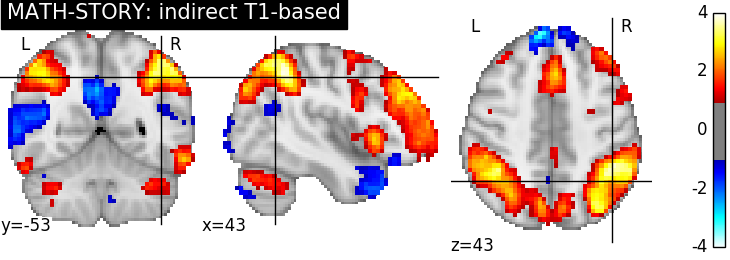
\includegraphics[width=.48\linewidth]{figures/MATH-STORY_DC+T1.png}
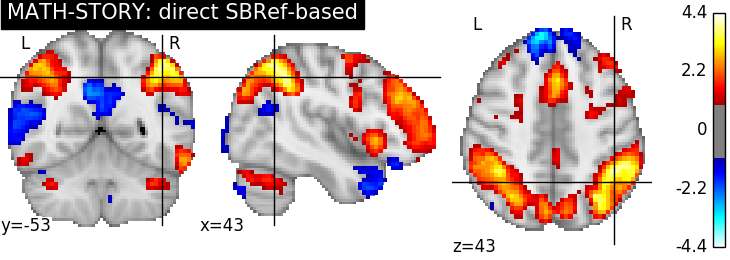
\includegraphics[width=.48\linewidth]{figures/MATH-STORY_DC+SBRef.png}
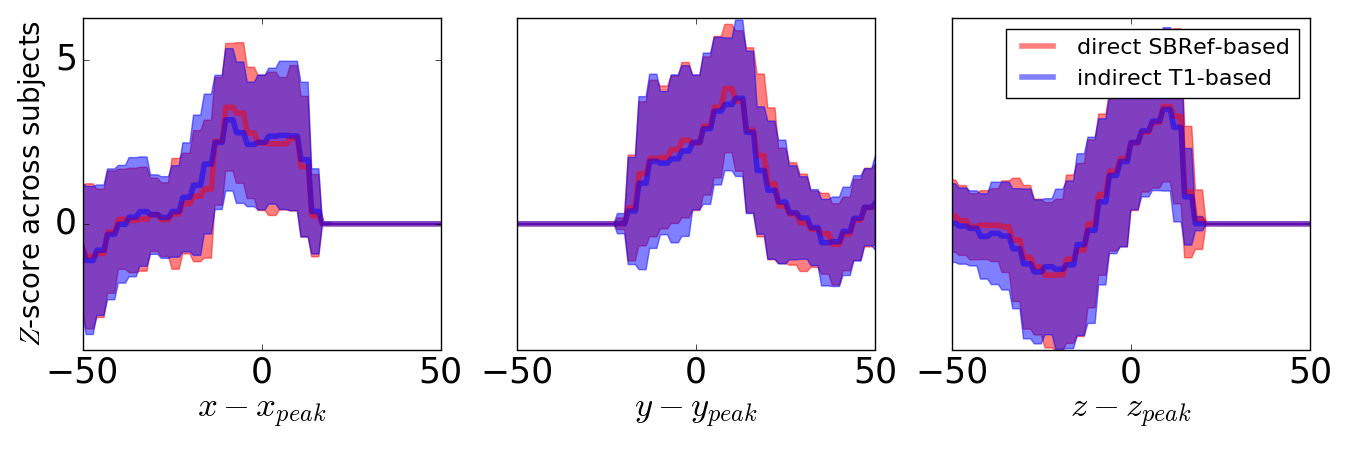
\includegraphics[width=1\linewidth]{figures/MATH-STORY_blobs.png}
\includegraphics[width=.48\linewidth]{figures/LH-RH_DC+T1.png}
\includegraphics[width=.48\linewidth]{figures/LH-RH_DC+SBRef.png}
\includegraphics[width=1\linewidth]{figures/LH-RH_blobs.png}

% \includegraphics[width=.48\linewidth]{figures/FACES-SHAPES_DC+T1.png}
% \includegraphics[width=.48\linewidth]{figures/FACES-SHAPES_DC+SBRef.png}
% \includegraphics[width=1\linewidth]{figures/FACES-SHAPES_blobs.png}
%% 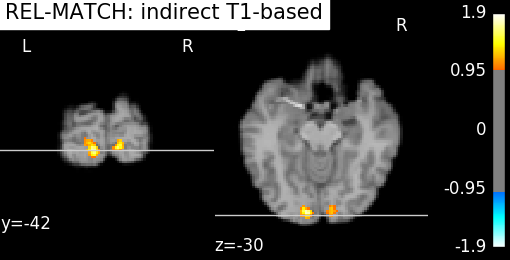
\includegraphics[width=.48\linewidth]{figures/REL-MATCH_DC+T1.png}
%% 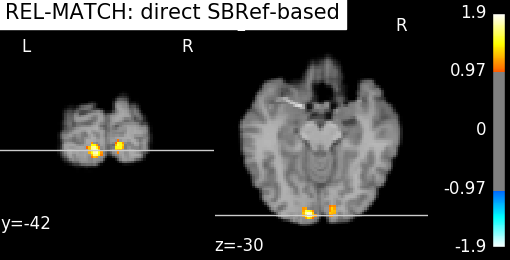
\includegraphics[width=.48\linewidth]{figures/REL-MATCH_DC+SBRef.png}
\includegraphics[width=.48\linewidth]{figures/LF-RF_DC+T1.png}
\includegraphics[width=.48\linewidth]{figures/LF-RF_DC+SBRef.png}
\includegraphics[width=1\linewidth]{figures/LF-RF_blobs.png}

%% \includegraphics[width=.48\linewidth]{figures/FACE-AVG_DC+T1.png}
%% \includegraphics[width=.48\linewidth]{figures/FACE-AVG_DC+SBRef.png}
%% \includegraphics[width=.48\linewidth]{figures/BODY-AVG_DC+T1.png}
%% \includegraphics[width=.48\linewidth]{figures/BODY-AVG_DC+SBRef.png}
% \includegraphics[width=.48\linewidth]{figures/TOM-RANDOM_DC+T1.png}
% \includegraphics[width=.48\linewidth]{figures/TOM-RANDOM_DC+SBRef.png}
% \includegraphics[width=1\linewidth]{figures/TOM-RANDOM_blobs.png}

\includegraphics[width=.48\linewidth]{figures/T-AVG_DC+T1.png}
\includegraphics[width=.48\linewidth]{figures/T-AVG_DC+SBRef.png}
\includegraphics[width=1\linewidth]{figures/T-AVG_blobs.png}

%% \includegraphics[width=.48\linewidth]{figures/REWARD-PUNISH_DC+T1.png}
%% \includegraphics[width=.48\linewidth]{figures/REWARD-PUNISH_DC+SBRef.png}
%% \includegraphics[width=.48\linewidth]{figures/TOOL-AVG_DC+T1.png}
%% \includegraphics[width=.48\linewidth]{figures/TOOL-AVG_DC+SBRef.png}
\caption{\textbf{Qualitative comparison} of pipelines via GLM results.
  Across-subject mean activation maps of $Z$-scores for different contrasts.
  Here we see that our proposed direct EPI-based registration scheme leads to slightly higher across-subject mean activation peaks.  For each contrast, a cut has been made around the location of the activation peak, to display curves of the activation profile and across-subject variability thereof, in a neighborhood of this peak location.
 %  \textbf{XXX: it'd be nice to give some names to the neuro-atomic landmarks visible in the above
 % activation maps (to add a neuroscientific flavour to the figure).}\textbf{XXX WDYM ? We can do that together whenever you want.}
}
\label{fig:zmaps}
\end{figure}

As regards group-level GLM scores, we see from Figure \ref{fig:zmaps}
that our proposed method does just as good as the classical indirect
T1-based pipeline. This is remarkable, as the former pipeline does not
use any anatomical data.
However, as noted in \citep{thirion2007analysis,pmid22425669}, the
inter-subject variability in GLM results is not due to
misregistration, but intrinsic subject differences with a more
physiological nature: the response of subjects to the same stimulus /
task is modulated differently, and is more dependent on effect size fluctuations than position. 

%
This
is confirmed in the curves in Figure \ref{fig:zmaps}, where we can see that the spatial across-subject activation profiles
are very similar between the compared registration methods, except for the already noted
slight improvement of the peak mean activation pattern obtained by our proposed method.

Finally, Figure \ref{fig:dmn} comparing the functional brain networks obtained by running
ICA on the images registered with each of the pipelines, shows essentially the same network
patterns. The absence of a difference between these maps can be explained by the fact that
resting state networks are less focal than task-based activation-patterns, and
so the former are less sensitive to the quality of the underlying registration procedure.

\section{Discussion and concluding remarks}
\label{sec:discussion}
Classical inter-subject registration pipelines use the T1 scan of a
subject to estimate the subject-to-template warp.
%
An obvious issue is that high-quality T1 scans are not always
available, but more generally, it is not always possible to completely
align the EPI images of a subject to their T1 image via
coregistration. Added to this is the possibility that such an intermediate registration step is
a potential source of interpolation artifacts, not to mention the added computational cost (which may exceed the rest of the computation time by many orders of magnitude, for example, in the case of surface-based methods). As shown by our experiments on the HCP dataset
\citep{VanEssen20122222} (Figure \ref{fig:pb_fig}), this is for example
the case in the presence of distortions
\citep{pmid9178246,pmid12270226,zeng2002,anderson2003} that persist
even after correction.  Further, as noted in \citep{pmid25405472},
distortions cannot be separated with registration based techniques,
which are compensatory operations. Consequently, the efficient
distortion correction method in EPI data remains an
open question. Our work proposes a direct EPI-based inter-subject
registration pipeline that to some extent evades these bottlenecks.

We have proposed a computationally cheap EPI-based pipeline for direct inter-subject nonlinear registration of functional data. Our method has been empirically validated on the HCP dataset \citep{VanEssen20122222}, where we have shown that we obtain registered subject images with less inter-subject variability. Such direct EPI-based methods should replace the well-accepted classical
T1-based strategy.
Results on the HCP dataset \citep{VanEssen20122222} show that the proposed pipeline outperforms the classical T1-based indirect registration strategy, according to a variety of different quality metrics: Normalized Mutual Information --NMI (Figure \ref{fig:nmi}), residual inter-subject
variance (Figure \ref{fig:cv}), and quality of estimated group template (Figure \ref{fig:template}), without compromising the quality of post-registration statistical analyses results (GLM, ICA, etc.).
These results replicate the findings of \citep{grabner2014} on a larger dataset (110 subjects, compared to 10 in the reference paper) and in a 3T setting.

\begin{pagefigure}
%   \includegraphics[width=.24\linewidth]{figures/DC+T1_AnteriormedialPFC.png}
% \includegraphics[width=.24\linewidth]{figures/DC+SBRef_AnteriormedialPFC.png}
% \includegraphics[width=.24\linewidth]{figures/DC+T1_Ventro-medialPFC.png}
% \includegraphics[width=.24\linewidth]{figures/DC+SBRef_Ventro-medialPFC.png}
% \includegraphics[width=.24\linewidth]{figures/DC+T1_Rightparahippocampalgyrus.png}
% \includegraphics[width=.24\linewidth]{figures/DC+SBRef_Rightparahippocampalgyrus.png}
% \includegraphics[width=.24\linewidth]{figures/DC+T1_PCC.png}
% \includegraphics[width=.24\linewidth]{figures/DC+SBRef_PCC.png}
\includegraphics[width=.48\linewidth]{figures/DC+T1_Leftlateralparietal.png}
\includegraphics[width=.48\linewidth]{figures/DC+SBRef_Leftlateralparietal.png}
\includegraphics[width=.48\linewidth]{figures/DC+T1_Rightlateralparietal.png}
\includegraphics[width=.48\linewidth]{figures/DC+SBRef_Rightlateralparietal.png}
% \includegraphics[width=.24\linewidth]{figures/DC+T1_Posteriorcingulate.png}
% \includegraphics[width=.24\linewidth]{figures/DC+SBRef_Posteriorcingulate.png}
\caption{Comparing functional brain networks from subject fMRI images registered with both pipelines, namely the classical indirect T1-based method, and our proposed direct EPI-based method). Shown here are group-level unthresholded sub-component maps of the Default Mode Network (DMN) \citep{raichle2001}, using MNI coordinates reported in Table 1 of \citep{Watanabe2013}.}
  \label{fig:dmn}
\end{pagefigure}

Remarkably, we observed that according to low-level QA metrics
like NMI (Figure \ref{fig:nmi}), residual inter-subject spatial
variability (Figure \ref{fig:cv}) and the  quality of across-subject mean
registered EPI image (Figure \ref{fig:template}), our proposes method
outperforms the classical indirect T1-based registration.
%
In terms of more high-level metrics like group-level GLM statistics, these gains though still present as not as pronounced (refer to Figure \ref{fig:zmaps}). Indeed, as noted in
\citep{thirion2007analysis,pmid22425669,Xu2009}, the inter-subject variability
in GLM results is not due to misregistration, but intrinsic subject
differences with a more physiological nature: the size of effects and
the anatomical localization are subject-specific. In chapter \ref{chap:rsfmri2tfmri},
we show that resting-state fMRI data can be used to predict the activation maps of
a subject to a task, with an $R^2$-score which can be up to \textbf{0.5} for some subjects and task.
This is an enhancement on previous work by \citep{tavor2016task}, and shows
differences in task-based brain activations are largely physiological --in contrast to being driven
by subjects' brain morphological differences-- and can be predicted from resting state fMRI data.

In a separate work \citep{dohmatob2016}, also presented in chapter \ref{chap:func_var} in detail, we have considered the possibility explicitly
modeling this physiology differences by estimating latent
factors of variability across-subjects in a data-driven way using
dictionary-learning. The motivating idea behind such a model, is that activation
across-subjects would be governed by the same generative model (the latent model),
and modulated on the subject-level by
subject-specific physiology. 

%% FInally, the misconception according to which function and anatomy
%% (i.e that accordingly, a local morphological variability could lead to a corre
%% sponding functional variability) are supposed to go hand in hand was further
%% destroyed in \citep{p}. They indeed tested
%% this hypothesis by linking the variability of the cortical
%% folding pattern of 252 right-handed subjects to the local-
%% ization or the pattern of functional activations induced by
%% hand motion or silent reading. Three regions are selected:
%% the central sulcus, the precentral sulcus and the superior
%% temporal sulcus (STS). ‘‘Essential morphological vari-
%% ability traits’’ are identified using a method building upon
%% multidimensional scaling. The link between variability in
%% anatomy and function is confirmed by the perfect match
%% between the central sulcus morphological ‘‘hand knob’’
%% and the corresponding motor activation: as the location

% Until the advent in the 1920s of non-invasive neuroimaging modalities, most of the accumulated knowledge of the brain came from the study of lesions, post-mortem analysis and invasive experimentations. With the advent of modern, non-invasive imaging techniques, several aspects of the human brain are revealed in vivo with high degree of precision.

% Several brain imaging techniques are available today. These can be divided into \emph{structural} or \emph{anatomical} and \emph{functional} imaging techniques. While structural imaging provides details on morphology and structure of tissues, functional imaging reveals physiological activities such as changes in metabolism, blood flow, regional chemical composition, and absorption. In this section we will discuss briefly the main functional neuroimaging modalities available today.

% \begin{itemize}
% \item{\bf {Electroencephalography - EEG}}
% % \begin{marginfigure}[3cm]
% % \center \includegraphics[width=.8\linewidth]{figures/eeg2.jpg}
% % \caption{EEG Cap}
% % \end{marginfigure}
% is a widely used modality for functional brain
% imaging. \emph{EEG} measures electrical activity along the scalp. EEG activity  reflects the synchronous activity of a population of neurons that have similar spatial orientation. If the cells do not have similar spatial orientation, their ions do not line up and thus do not create detectable waves. Pyramidal neurons of the cortex are thought to produce most of the EEG signals because they are well-aligned and fire together. Because voltage fields fall off with the square of distance, activity from deep sources is more difficult to detect than currents near the skull. Due to the ill-posed problem of
% volumetric data reconstruction from surface measurements,
% \emph{EEG} has a poor spatial resolution compared to other modalities
% such as \emph{fMRI}.

% \item{\bf {Stereotactic electroencephalography - sEEG}} is an invasive version of
% \emph{EEG}, based on intra-cranial recording. It measures the electrical
% currents
% within some regions of the brain using deeply implanted electrodes, localized
% with a stereotactic technique.
% This approach has the good temporal resolution of \emph{EEG} and enjoys an
% excellent spatial resolution. However, \emph{sEEG}
% is very invasive and is only performed for medical purpose (\emph{e.g}
% localization of epilepsy foci) and has a limited coverage (only the regions with electrodes).
% A close approach is \emph{Electrocorticography -- ECog --} that uses
% electrodes placed directly on the exposed surface of the brain. Even in this case its usage is restricted to medical purposes.


% \begin{marginfigure}[5cm]
% \center \includegraphics[width=1.\linewidth]{chapter_1/meg.pdf}
% \caption{Magnetic field measured with MEG on a somato-sensory experiment. It is a 2D topography 20 ms after stimulation. Source: \citep{gramfort:09}}
% \end{marginfigure}
% \item{\bf{Magnetoencephalography - MEG}}
% measures the magnetic field induced by neural electrical activity.
% The synchronized currents in neurons create magnetic fields of a
% few hundreds of femto Tesla ($fT$) that can be detected using specific devices. 
% Although EEG and MEG signals originate from the same neurophysiological processes, there are important differences. Magnetic fields are less distorted than electric fields by the skull and scalp, which results in a better spatial resolution of the MEG. Whereas EEG is sensitive to both tangential and radial components of a current source in a spherical volume conductor, MEG detects only its tangential components. Because of this EEG can detect activity both in the sulci and at the top of the cortical gyri, whereas MEG is most sensitive to activity originating in sulci. EEG is, therefore, sensitive to activity in more brain areas, but activity that is visible in MEG can be localized with more accuracy. Note that EEG and MEG can be measured simultaneously.


% \item{\bf{Positron emission tomography - PET}}
%  is an imaging modality based on the
% detection of a radioactive tracers introduced in the body of the subject. The
% tracers (or \emph{radionuclide} decay) emit a positron which can in turn emit,
% after recombination with an electron, a pair of photons that are detected
% simultaneously. PET therefore provides a quantitative measurement of the physiological activity. It can also be used for functional imaging, by choosing a specific tracer.
% In particular, the \emph{fluorodeoxyglucose} (or \emph{FDG}), is used for
% imaging the metabolic activity of a tissue. This is based on the assumption that areas of high radioactivity are associated with brain activity.
% \emph{PET} has two major limitations: the tracers required for
% \emph{PET} are produced by cyclotrons (a type of particle accelerator),
% which implies an heavy logistic. Furthermore, the use of radio-tracers is not harmless
% for the
% health of the subjects so \emph{PET} is now used for medical purpose only.

% \begin{marginfigure}[0cm]
% \center \includegraphics[width=.8\linewidth]{chapter_1/212px-PET-image.jpg}
% \caption{PET scan of a human brain. 
% PET measures indirectly the flow of blood to different parts of the brain, which is, in general, believed to be correlated with neural activity.
% Souce: wikipedia.org}
% \end{marginfigure}


% \item{\bf{Single photon emission computed tomography - SPECT}} is an imaging modality based on the detection of a radioactive tracer. SPECT is similar
% to \emph{PET} in its use of radioactive tracer material. However, the
% measure in \emph{SPECT} is the direct consequence of the tracer (the tracer
% emits gamma radiation), where \emph{PET} is based on an indirect consequence of
% the tracer (positron then gamma radiation). The spatial resolution is slightly worse
% than \emph{PET}.
% %
% \emph{SPECT} can be used for functional brain imaging, by using a specific
% tracer which will be assimilated by the tissue in an amount proportional to
% the cerebral blood flow.


% \item{\bf{Near-infrared spectroscopy - nIRS}}
%  is a recent modality for
% medical imaging. \emph{nIRS} is based on the fact that the absorption of the
% light in the
% near-infrared domain contains information on the blood flow and blood
% oxygenation level. It is non-ionizing (harmless), and the instruments are
% not too expensive. However, the spectra obtained by \emph{nIRS} can be difficult
% to interpret, and this technique, which requires a complex calibration, measures
% signals only close to the outer layer of the cortex.

% \newglossaryentry{fMRI}{name=fMRI,description=Functional Magnetic Resonance Imaging}

% \item{\bf{Functional MRI} -- {\gls{fMRI}}} is
% a widely used method for functional brain imaging, because it is
% non-invasive, has a good spatial
% resolution ($1mm^3$), and provides access,
% albeit indirectly, to the neural activity.
% Moreover, in standard acquisitions, \emph{fMRI} yields a
% full-brain coverage, as it does not
% restrict the study to superficial layers or predefined regions of the cortex.

% \end{itemize}


% Different modalities have different trade offs in terms of spatial and temporal resolution. For example, EEG and MEG enjoy temporal resolutions of the order of few miliseconds and are thus well suited for studies of temporal dynamics of information processing but have limited spatial resolution. On the other hand, fMRI enjoys a better spatial resolution but the temporal resolution is around 1 second. Furthermore, as we will see in the next section, temporal resolution in fMRI is further limited by the slow spread of hemodynamic response, which lasts around 20 seconds after the stimuli presentation.




% \begin{figure}[h!tb]
% \center \includegraphics[width=0.8\linewidth]{chapter_1/chapter_1_methods.pdf}
% \caption[Spatial and temporal resolutions of the different modalities commonly
% used for functional imaging]{Spatial and temporal resolutions of different
% modalities commonly
% used for functional imaging. A typical fMRI acquisition (as of 2014) enjoys spatial resolution of the order of {$1-3mm^3$} and temporal resolution of the order of 1-3 seconds.}\label{fig:chapter1_methods}
% \end{figure}

% Certain imaging techniques are more adapted than other to answer certain neuroscientific questions. Due to its good spatial resolution and whole brain coverage, fMRI is particularly well adapted to \emph{localize} the effect of a certain experimental condition. This task is not reduced to the construction of brain maps, but also involves the understanding of the underlying brain connectivity~\citep{johansen2005functional,behrens2006consistent} and the effects regions exert on each other in a certain experimental context~\citep{pessiglione2007brain, behrens2007learning}. One of the main hopes in functional imagining is that it might be used as an objective diagnosis tool for several diseases. In particular, the aim is to find some \emph{biomarkers} for psychiatric diseases by comparing different population of patients: this is the case for autism, schizophrenia or Alzheimer's disease. 

% \clearpage
\bibliographystyle{plainnat}
\bibliography{bib_all}





